\PassOptionsToPackage{unicode=true}{hyperref} % options for packages loaded elsewhere
\PassOptionsToPackage{hyphens}{url}
%
\documentclass[]{article}
\usepackage{lmodern}
\usepackage{setspace}
\setstretch{2}
\usepackage{amssymb,amsmath}
\usepackage{ifxetex,ifluatex}
\usepackage{fixltx2e} % provides \textsubscript
\ifnum 0\ifxetex 1\fi\ifluatex 1\fi=0 % if pdftex
  \usepackage[T1]{fontenc}
  \usepackage[utf8]{inputenc}
  \usepackage{textcomp} % provides euro and other symbols
\else % if luatex or xelatex
  \usepackage{unicode-math}
  \defaultfontfeatures{Ligatures=TeX,Scale=MatchLowercase}
\fi
% use upquote if available, for straight quotes in verbatim environments
\IfFileExists{upquote.sty}{\usepackage{upquote}}{}
% use microtype if available
\IfFileExists{microtype.sty}{%
\usepackage[]{microtype}
\UseMicrotypeSet[protrusion]{basicmath} % disable protrusion for tt fonts
}{}
\IfFileExists{parskip.sty}{%
\usepackage{parskip}
}{% else
\setlength{\parindent}{0pt}
\setlength{\parskip}{6pt plus 2pt minus 1pt}
}
\usepackage{hyperref}
\hypersetup{
            pdftitle={Physcraper: a python package for continual update of evolutionary estimates using the Open Tree of Life},
            pdfborder={0 0 0},
            breaklinks=true}
\urlstyle{same}  % don't use monospace font for urls
\usepackage[margin = 1in]{geometry}
\usepackage{longtable,booktabs}
% Fix footnotes in tables (requires footnote package)
\IfFileExists{footnote.sty}{\usepackage{footnote}\makesavenoteenv{longtable}}{}
\usepackage{graphicx,grffile}
\makeatletter
\def\maxwidth{\ifdim\Gin@nat@width>\linewidth\linewidth\else\Gin@nat@width\fi}
\def\maxheight{\ifdim\Gin@nat@height>\textheight\textheight\else\Gin@nat@height\fi}
\makeatother
% Scale images if necessary, so that they will not overflow the page
% margins by default, and it is still possible to overwrite the defaults
% using explicit options in \includegraphics[width, height, ...]{}
\setkeys{Gin}{width=\maxwidth,height=\maxheight,keepaspectratio}
\setlength{\emergencystretch}{3em}  % prevent overfull lines
\providecommand{\tightlist}{%
  \setlength{\itemsep}{0pt}\setlength{\parskip}{0pt}}
\setcounter{secnumdepth}{5}
% Redefines (sub)paragraphs to behave more like sections
\ifx\paragraph\undefined\else
\let\oldparagraph\paragraph
\renewcommand{\paragraph}[1]{\oldparagraph{#1}\mbox{}}
\fi
\ifx\subparagraph\undefined\else
\let\oldsubparagraph\subparagraph
\renewcommand{\subparagraph}[1]{\oldsubparagraph{#1}\mbox{}}
\fi

% set default figure placement to htbp
\makeatletter
\def\fps@figure{htbp}
\makeatother

\usepackage{color}
\usepackage{hyperref}
\usepackage{caption}
\usepackage{blindtext}
\usepackage{url}
\usepackage[left]{lineno}
\linenumbers

\title{Physcraper: a python package for continual update of evolutionary estimates using the Open Tree of Life}
\author{}
\date{\vspace{-2.5em}}

\begin{document}
\maketitle

\textbf{1. Luna L. Sanchez Reyes}

School of Natural Sciences, University of California, Merced

email: \href{mailto:sanchez.reyes.luna@gmail.com}{\nolinkurl{sanchez.reyes.luna@gmail.com}}

\textbf{2. Martha Kandziora}

School of Natural Sciences, University of California, Merced

email: \href{mailto:martha.kandziora@mailbox.org}{\nolinkurl{martha.kandziora@mailbox.org}}

\textbf{3. Emily Jane McTavish}

School of Natural Sciences, University of California, Merced

email: \href{mailto:ejmctavish@gmail.com}{\nolinkurl{ejmctavish@gmail.com}}

\textbf{Correspondence address}: Science and Engineering Building 1, University of California, Merced, 5200 N. Lake Rd, Merced CA 95343

\textbf{Correspondence email}: \href{mailto:sanchez.reyes.luna@gmail.com}{\nolinkurl{sanchez.reyes.luna@gmail.com}}, \href{mailto:ejmctavish@gmail.com}{\nolinkurl{ejmctavish@gmail.com}}

\textbf{Running title}: Continually updated gene trees with Physcraper

\textbf{Word count}: 3073

\textbf{Manuscript prepared for submission to Methods in Ecology and Evolution}

\textbf{Article type}: Application

\newpage

\hypertarget{abstract}{%
\section{Abstract}\label{abstract}}

\begin{enumerate}
\def\labelenumi{\arabic{enumi}.}
\item
  Phylogenies are a key part of research in all areas of biology. Tools that automatize
  some parts of the process of phylogenetic reconstruction (mainly character matrix construction)
  have been developed for the advantage of both specialists in the field of phylogenetics and nonspecialists.
  However, interpretation of results, comparison with previously available phylogenetic
  hypotheses, and choosing of one phylogeny for downstream analyses and discussion still impose difficulties
  to one that is not a specialist either on phylogenetic methods or on a particular group of study.
\item
  Physcraper is an open‐source, command-line Python program that automatizes the update of published
  phylogenies by making use of public DNA sequence data and taxonomic information,
  providing a framework for comparison of published phylogenies with their updated versions.
\item
  Physcraper can be used by the nonspecialist, as a tool to generate phylogenetic
  hypothesis based on already available expert phylogenetic knowledge.
  Phylogeneticists and group specialists will find it useful as a tool to facilitate comparison
  of alternative phylogenetic hypotheses (topologies).
  \textbf{\emph{Is physcraper intended for the nonspecialist?? We have two types of nonspecialists:
  the ones that do not know about phylogenetic methods and the ones that might know
  about phylogenetic methods but do not know much about a certain biological group.}}
\item
  Physcraper implements node by node/topology comparison of the the original and the updated
  trees using the conflict API of OToL, and summarizes differences.
\item
  We hope the physcraper workflow demonstrates the benefits of opening results in phylogenetics and encourages researchers to strive for better data sharing practices.
\item
  Physcraper can be used with any OS. Detailed instructions for installation and
  use are available at \url{https://github.com/McTavishLab/physcraper}.
\end{enumerate}

\textbf{Keywords}: cross-connectivity, gene tree, open science, open tree of life, phylogeny, public database, python, reproducibility, taxonomy, updated alignment

\newpage

\hypertarget{introduction}{%
\section{Introduction}\label{introduction}}

From molecular data to alignments and phylogenies, public biological data repositories such as the GenBank database (Benson \emph{et al.} \protect\hyperlink{ref-benson2000genbank}{2000}; Wheeler \emph{et al.} \protect\hyperlink{ref-wheeler2000database}{2000}), the TreeBASE repository (Piel \emph{et al.} \protect\hyperlink{ref-piel2009treebase}{2009}) and the Open Tree of Life curating system (McTavish \emph{et al.} \protect\hyperlink{ref-mctavish2015phylesystem}{2015}), are still accumulating data.

More than a decade ago, the National Center for Biodiversity Information (NCBI) molecular database, GenBank, released its version number 159 (April 15, 2007). With 72 million DNA sequences, it was estimated to have the potential to resolve evolutionary relationships of most of the 241 000 distinct taxa represented in it (about 98.05\% of taxa in the NCBI taxonomy; Sanderson \emph{et al.} \protect\hyperlink{ref-sanderson2008phylota}{2008}), covering about 10\% of extant described biodiversity (taking a conservative estimate of extant diversity; Scott \protect\hyperlink{ref-scott2011ncbi}{2011}; Federhen \protect\hyperlink{ref-federhen2003taxonomy}{2003}).
In comparison, the current GenBank release number 238 (June 15, 2020) has tripled in size, hosting data for more than 217 million DNA sequences \url{https://ftp.ncbi.nih.gov/genbank/gbrel.txt}.

Many useful tools have been developed in the past decades in an effort to make sense of the large amount of data in public molecular databases, as well as private ones. Generally refered to as ``pipelines'', most of these tools were motivated by the genomics revolution, to identify clusters of homologs for genomic assembly. Notably, this homolog DNA clusters can be used as homology hypotheses (aka molecular alignments) to reconstruct phylogenetic relationships.
Pipelines that automatize the assembly of DNA alignments from the GenBank database for phylogenetic reconstruction (refered to as ``phylogenetic pipelines'') such as PHYLOTA (Sanderson \emph{et al.} \protect\hyperlink{ref-sanderson2008phylota}{2008}), PHLAWD (Smith \emph{et al.} \protect\hyperlink{ref-smith2009mega}{2009}), and SUPERSMART (Antonelli \emph{et al.} \protect\hyperlink{ref-antonelli2017toward}{2017}), have been widely used to study the evolutionary relationships among different organisms (TABLE?? maybe supplementary data), from a phylogeny of no more than 20 species of the family of barracuda fish (Sphyraenidae; Santini \& Sorenson \protect\hyperlink{ref-santini2013first}{2013}), to a mega-phylogeny of almost 3 000 species of living ferns (Lehtonen \protect\hyperlink{ref-lehtonen2011towards}{2011}).

Pipelines have been an important incorporation to the field of phylogenetics in many ways, particularly because they represent a clear step towards reproducibility in the field. In contrast, most published phylogenies have been infered using homology hypotheses that have been curated ``by hand'' (Morrison \protect\hyperlink{ref-morrison2009would}{2009}).
What explains this preference? aka the discordance between the genomics approach (a gazillion markers poorly aligned, but the amount of data will overcome errors in alignment) and the classic phylogenetics approach (few markers thoughtfully curated).
On one hand, there are concerns about the use of automated pipelines in phylogenetics.
Concerns I think people have about these tools:
- Errors in identification of sequences
- Little control at different steps of the process
- Too much of a black box? Most of these phylogenies are being constructed by people learning about the methods (aka students), so they want to know what is going on at each step and end up doing it manually.
-
It has also been suggested that manual curation of classic and genomic alignments produces better phylogenetic reconstructions (Fragoso-Martínez \emph{et al.} \protect\hyperlink{ref-fragoso2017pilot}{2017}).

A way to incorporate the best of two worlds (massive amounts of newly released molecular data VS fine curation from human experts) would be to rely on published manually curated homology hypotheses. This expert-curated alignments can be enriched and updated by incorporating newly released data from public molecular databases.

As of April 2014, TreeBASE hosted a bit more than 8 200 curated alignments, providing information on evolutionary relationships of almost 105 000 distinct taxa \href{https://www.treebase.org/treebase-web/home.html\#:~:text=TreeBASE\%20is\%20produced\%20and\%20governed,mapped\%20to\%20104\%2C593\%20distinct\%20taxa.}{(see TreeBASE about)}.
This provides an untapped source of valuable knowledge with the potential to update phylogenetic relationships in different regions of the tree of life.

The OToL tree repository (phylesystem; McTavish \emph{et al.} \protect\hyperlink{ref-mctavish2015phylesystem}{2015}) automatically incorporates the phylogenies from TreeBASE, and stores metadata linking the tree to its corresponding alignment repository in TreeBASE. This provides a loose means of linking the tree with the exact alignment that generated it. This can be a difficult task when multiple alignments were originally deposited and no clear link between alignment and tree was provided in TreeBASE.

Ultimately, linkage of original alignment with its corresponding phylogeny has to be done by a human curator.
Moreover, each one of these data repositories follow their own system for taxon identification. A real challenge is to find an effective way to link data from across databases that belongs to the same taxon.
OToL's metadata system incorporates taxon identifiers from a variety of taxonomies and repositories, including the NCBI taxonomy, GBIF, etc.

Physcraper is a python pipeline that uses the OToL metadata system to connect databases through taxon identification numbers.

It's main goal is to connect public phylogenetic relationships in OToL, with alignments from TreeBASE and GenBank DNA data.

It also allows automatizing and standardizing the comparison of phylogenetic hypotheses.

This is an effort to keep on directing ourselves towards a fully reproducible workflow in phylogenetics.
And an effort to more effectively connect the world of big data in biology.

\hypertarget{how-does-physcraper-work}{%
\section{How does Physcraper work?}\label{how-does-physcraper-work}}

\hypertarget{the-input-a-study-tree-and-an-alignment}{%
\subsection{The input: a study tree and an alignment}\label{the-input-a-study-tree-and-an-alignment}}

\begin{itemize}
\tightlist
\item
  The study tree is a published phylogenetic tree stored in the OToL database, phylesystem (McTavish \emph{et al.} \protect\hyperlink{ref-mctavish2015phylesystem}{2015}). The main
  reason for this is that trees in phylesystem have a set of user defined characteristics
  that are essential for automatizing the phylogeny update process. The most relevant of these being the definition of ingroup and outgroup. Outgroup and ingroup taxa in the original tree are identified and tagged. This allows to automatically set the root for the updated tree on the next steps of the pipeline.
  A user can choose from the 1216 published trees supporting the resolved node of the synthetic tree in the OToL website (\textless{}\textgreater{}). If the tree you are interested in updating is not in there, you can upload it via OToL's curator tool (\textless{}\url{https://tree.opentreeoflife.org/curator}).
\item
  The alignment should be a gene alignment that was used to generate the tree. The original
  alignments are usually stored in a public repository such as TreeBase (Piel \emph{et al.} \protect\hyperlink{ref-piel2009treebase}{2009}; Vos \emph{et al.} \protect\hyperlink{ref-vos2012nexml}{2012}),
  DRYAD (\url{http://datadryad.org/}), or the journal were the tree was originally published.
  If the alignment is stored in TreeBase, \texttt{physcraper} can download it directly,
  either from the TreeBASE website (\url{https://treebase.org/})
  or through the TreeBASE GitHub repository (SuperTreeBASE; \url{https://github.com/TreeBASE/supertreebase}).
  If the alignment is on another repository, or provided personally by the owner, a copy of it has to be
  downloaded by the user, and it's local path has to be provided as an argument.
\item
  A taxon name matching step is performed to verify that all taxon names on the tips
  of the tree are in the DNA character matrix and vice versa.
\item
  A ``.csv'' file with the summary of taxon name matching is produced for the user.
\item
  Unmatched taxon names are dropped from both the tree and alignment.
  Technically, just one matching name is needed to perform the searches. Please, see next section.
\item
  A ``.tre'' file and a ``.fas'' file containing only the matched taxa are generated and saved in the \texttt{inputs} folder to be used in the following steps.
\end{itemize}

\hypertarget{dna-sequence-search-and-cleaning}{%
\subsection{DNA sequence search and cleaning}\label{dna-sequence-search-and-cleaning}}

\begin{itemize}
\item
  The next step is to identify the search taxon within the reference taxonomy. The search taxon will be used to constraint the DNA sequence search on the nucleotide database within that taxonomic group. Because we are using the NCBI nucleotide database, by default the reference taxonomy is the NCBI taxonomy. The search taxon can be provided by the user. If none is provided, then the search taxon is identified as the Most Recent Common Ancestor (MRCA) of the
  matched taxa belonging to the ingroup in the tree, that is also a named clade in the reference taxonomy. This is known as the Most Recent Common
  Ancestral Taxon (MRCAT; also referred in the literature as the Least Inclusive Common Ancestral Taxon - LICA).
  The MRCAT can be different from the phylogenetic MRCA when the latter is an unnamed clade in the reference taxonomy.
  To automatically identify the MRCAT of a group of taxon names, we make use of the OToL taxonomy tool (\url{https://github.com/OpenTreeOfLife/germinator/wiki/Taxonomy-API-v3\#mrca}).

  Users can provide a search taxon that is either a more or a less inclusive
  clade relative to the ingroup of the original phylogeny. If the search taxon is more inclusive, the sequence search will be performed outside the MRCAT of the matched taxa, e.g., including all taxa within
  the family or the order that the ingroup belongs to. If the search taxon is a less inclusive clade, the users can focus on enriching a particular clade/region within the ingroup of the phylogeny.
\item
  The Basic Local Alignment Search Tool, BLAST {[}Altschul \emph{et al.} (\protect\hyperlink{ref-altschul1990basic}{1990}); altschul1997gapped{]} is used to identify
  similarity between DNA sequences within the search taxon in a nucleotide
  database, and the accepted sequences on the alignment.
  The blastn function from the BLAST command line tools (Camacho \emph{et al.} \protect\hyperlink{ref-camacho2009blast}{2009}) is used for local-database searches.
  A modified biopython blast function is used for web-based searches.
\item
  The DNA sequence similarity search can be done on a local database that is easily
  setup by the user. In this case, the blastn function is used to performs the similarity search (Camacho \emph{et al.} \protect\hyperlink{ref-camacho2009blast}{2009}).
\item
  The search can also be performed remotely, on the NCBI database. In this case, the
  bioPython BLAST function was modified to accepts is used to perform the similarity search.
\item
  A pairwise alignment-against-all BLAST search is performed. This means that each sequence
  in the alignment is BLASTed against DNA sequences in a nucleotide database constrained to the search
  taxon. Results from each one of these BLAST runs are recorded, and matched sequences are saved
  along with their corresponding identification numbers (accesion numbers in the case of the GenBank database). This information will be used later to store the whole sequences in a dedicated library within the physcraper folder, allowing for secondary analyses to run significantly faster.
\item
  Matched sequences below an e-value, percentage similarity, and outside a minimum
  and maximum length threshold are discarded. \textbf{\emph{REPORT THE DEFAULT VALUES AND DESCRIBE WHAT THEY MEAN}} This filtering leaves out genomic sequences.
  All acepted sequences are asigned an internal identifier, and are further filtered.
\item
  Because the original alignments usually lack database id numbers, a filtering
  step is needed. Accepted sequences that belong to the
  same taxon of the query sequence, and that are either identical or shorter than
  the original sequence are discarded. Only longer sequences belonging to the
  same taxon as the orignal sequence will be considered further for analysis.
\item
  Among the remaining filtered sequences, there are usually several exemplars per taxon.
  Although it can be useful to keep some of them to, for example, investigate monophyly
  within species, there can be hundreds of exemplar sequences per taxon for some markers.
  To control the number of sequences per taxon in downstream analyses,
  5 sequences per taxon are chosen at random. This number is set by default but can be modified by the user.
\item
  Reverse complement sequences are identified and translated.
\item
  Users can choose to perform a more ``cycles'' of sequence similarity search, by blasting the newly found sequences. This can be done iteratively, but by default only sequences in the alignment are blasted. \textbf{\emph{Is there an argument to control the number of cycles of blast searches with new sequences?}}
\item
  Accepted sequences are downloaded in full, and stored as a local database in a directory that is globally accesible (physcraper/taxonomy), so they are accesible for further runs.
\item
  A fasta file containing all filtered and processed sequences resulting from the BLAST search is generated for the user.
\end{itemize}

\hypertarget{dna-sequence-alignment}{%
\subsection{DNA sequence alignment}\label{dna-sequence-alignment}}

\begin{itemize}
\tightlist
\item
  The software MUSCLE (Edgar \protect\hyperlink{ref-edgar2004muscle}{2004}) is implemented to perform alignments.
\item
  First, all new sequences are aligned using default MUSCLE options.
\item
  Then, a MUSCLE profile alignment is performed, in which the original alignment
  is used as a template to align new sequences. This ensures that the final alignment
  follows the homology criteria established by the original alignment.
\item
  The final alignment is not further processed automatically. We encourage users
  to check it either by eye and perform manual refinement or using any of the many
  tools for alignment processing, to eliminate columns with no information.
\end{itemize}

\hypertarget{tree-reconstruction-and-comparison}{%
\subsection{Tree reconstruction and comparison}\label{tree-reconstruction-and-comparison}}

\begin{itemize}
\item
  A gene tree is reconstructed for each alignment provided, using a Maximum Likelihood approach implemented with the software RAxML (Stamatakis \protect\hyperlink{ref-stamatakis2014raxml}{2014})
  with 100 classic rapid bootstrap (Felsenstein \protect\hyperlink{ref-felsenstein1985confidence}{1985}) replicates by default. The number of bootsrap replicates can be modified by the user.
  Other type of bootstrap that I think is not yet incorporated into physcraper is the Transfer Bootstrap Expectation (TBE) recently proposed in Lemoine \emph{et al.} (\protect\hyperlink{ref-lemoine2018renewing}{2018}).
\item
  The original tree is used as starting tree for the ML searches. It can also be set as a full topological constraint or not used at all, depending on the goals of the user.
\item
  Bootstrap results are summarized with Dendropy ADD CITATION
\item
  The final result is an updated phylogenetic hypothesis for each of the genes provided in the alignment.
\item
  Tips on all trees generated by physcraper are defined by a taxon name space, allowing to perform comparisons and conflict analyses.
\item
  Robinson Foulds weighted and unweighted metrics ARE CALCULATED WITH DENDROPY TOO.
\item
  Describe what a conflict analysis is: Node by node comparison between the original and updated tree, and the synthetic OToL using the conflict API of otol CITE REDELINGS AND HOLDER ({\textbf{???}} and holder).
\item
  For the conflict analysis to be meaningful, the root of the tree ineeds to be accurately defined.
\item
  A SUGGESTED DEFAULT ROOTING BASED ON THE OPEN TREE TAXONOMY is implemented for now. DESCRIBE HOW IT WORKS. SAY THAT IT IS A PROBLEM. Automatic rooting is not that smart yet. The best way right now is for users to define outgroups so trees are better rooted.
\item
  Currently, the root is determined by finding the parent node of the sequences that do not belong to the ingroup/ search taxon. This ensures a correct rooting of the tree even when the search taxon is more inclusive than the ingroup.
\item
  Conflict information can only be generated in the context of the whole Open Tree of
  Life. Otherwise, it is not really possible to get conflict data.
  \textbf{\emph{- One way to compare two independent phylogenetic trees is to compare them both to
  the synthetic OToL and then measure how well they do against each other}}
\end{itemize}

\hypertarget{examples}{%
\section{Examples}\label{examples}}

To exemplify the utility of physcraper we will address two use-case scenarios. One in which the user is interested in a particular group. Another one in which the user is interested in a particular phylogeny.
A tutrial as well as illustrated examples of steps needed to perform a physcraper analyses are available elsewhere.

\hypertarget{the-hollies}{%
\subsection{The hollies}\label{the-hollies}}

A student is interested in the genus \emph{Ilex}, the only extant clade within the family Aquifoliaceae, order Aquifoliales of flowering plants.
The genus encompasses between 400-600 living species. A review of literature reveals that there are three phylogenetic trees showing relationships within the hollies published.
The first one has been made available in TreeBASE as well as in the OToL phylesystem and is part of the synthetic tree. It samples 48 species.
The second tree has not been made available anywhere, not even in the supplementary data of the original publication.
The most recent one has been made available in the OToL Phylesystem and in the DRYAD repository. It is the best sampled yet, with 200 species. However, it has not been added to the syntehtic tree yet.
This makes it a perfect case to test the basic functionalities of physcraper: we know that the sequences of the most recently published tree have been made available on the GenBank database. Hence, we expect that updating the oldest tree will produce something very similar to the newest tree.

\hypertarget{the-malvaceae}{%
\subsection{The Malvaceae}\label{the-malvaceae}}

A postdoc started working with a new reserach group. They are interested in solving relationships among lineages of the Malvaceae, a family of flowering plants with almost 6 000 known species.
A review of the literature shows them that there are many phylogenetic trees encompassing some of the linegaes in the group. However, the head of the group wants to use a particular marker they beilieve to be the best one to be able to solve the relationships in the group. They have been working in the alignment for long and they want to incorporate new data into the hypothesis of homology they have been curating and that they trust.

\begin{figure}

{\centering 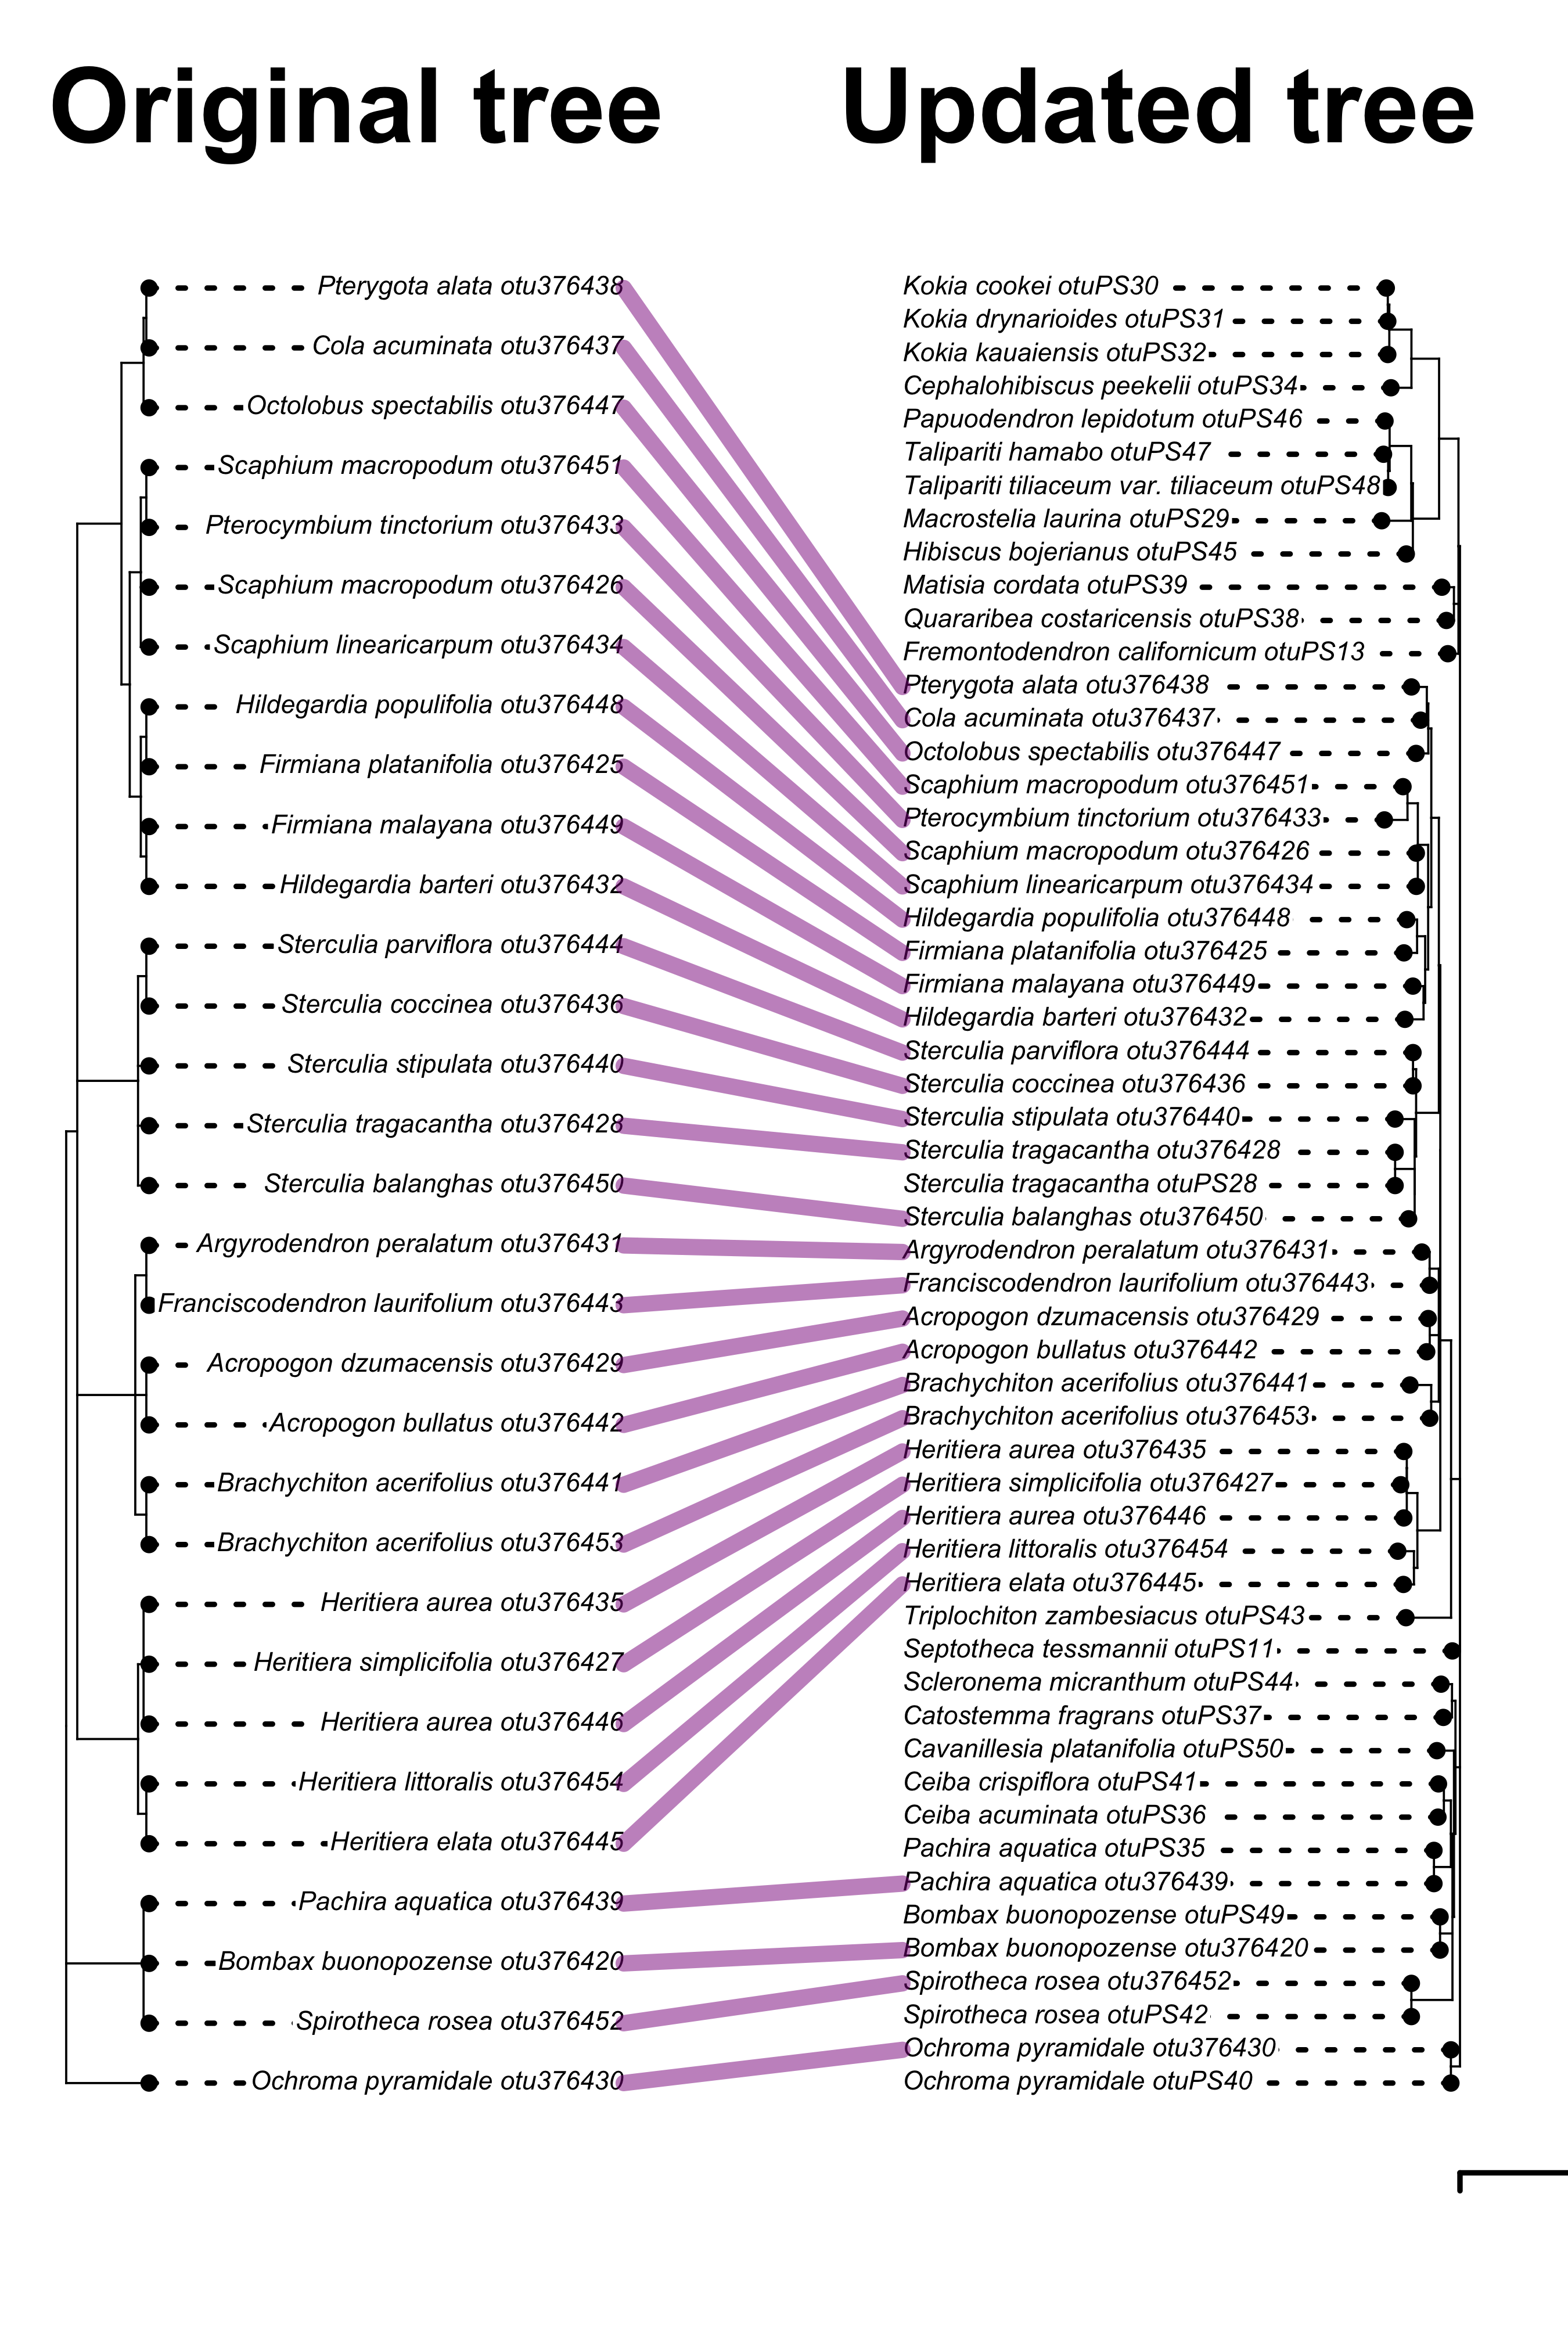
\includegraphics[width=0.85\linewidth]{docs/figs/cotree-plot2-1} 

}

\caption{Comparison of original tree and update tree of the Malvaceae.}\label{fig:fig-2}
\end{figure}
\newpage

\hypertarget{discussion}{%
\section{Discussion}\label{discussion}}

Data repositories hold more information than meets the eye.
Besides the actual data, they have other types of information that can be used for the advantage of science.

Usually, initial ideas about the data are changed by analyses.
We expect that this new ideas on the data can be registered on data bases,
exposing new comers to expert understanding about the data.

There are many tools that are making use of DNA data repositories in different ways.
Most of them focus on efficient ways to mine the data -- getting the most homologs.
Some focus on accurate ways of mining the data - getting real and clean homologs.
Others focus on refinement of the alignment.
Most focus on generating full trees \emph{de novo}, mainly for regions of the Tree of
Life that have no phylogenetic assessment yet in published studies, but also for
regions that have been already studied and that have phylogenetic data already.

All these tools are great efforts for advancing towards reproducibility in phylogenetics,
a field that has been largely recognised as somewhat artisanal.
We propose adding focus to other sources of information available from data repositories.
Taking advantage of public DNA data bases have been the main focus. However, phylogenetic knowledge is
also accumulating fast in public and open repositories.
In this way, the physcraper pipeline can be complemented with other tools that have
been developed for other purposes.

We emphasize that physcraper takes advantage of the knowledge and intuition of the expert
community to build upon phylogenetic knowledge, using not only data accumulated in
DNA repositories, but phylogenetic knowledge accumulated in tree repositories.
This might help generate new phylogenetic data. But physcraper does not seek to generate full phylogenies \emph{de novo}.

Describe again statistics to compare phylogenies provided by physcraper via OpenTreeOfLife.
Mention statistics provided by other tools: PhyloExplorer (Ranwez \emph{et al.} \protect\hyperlink{ref-ranwez2009phyloexplorer}{2009}).
Compare and discuss.

How is physcraper already useful:
- to mine targeted sequences, in this way it is similar to baited analyses from PHLAWD and pyPHLAWD. Phylota does not do baited analyses, I think, only clustered analyses.
- Finding

How can it be used for the advantage of the field:
- rapid phylogenetic placing of newly discovered species, as mentioned in Webb \emph{et al.} (\protect\hyperlink{ref-webb2010biodiversity}{2010})
- obtain trees for ecophylogenetic studies, as mentioned in Helmus \& Ives (\protect\hyperlink{ref-helmus2012phylogenetic}{2012})
- one day could be used to sistematize nucleotide databases, such as Genbank (Benson \emph{et al.} \protect\hyperlink{ref-benson2000genbank}{2000}; Wheeler \emph{et al.} \protect\hyperlink{ref-wheeler2000database}{2000}), as mentioned in San Mauro \& Agorreta (\protect\hyperlink{ref-san2010molecular}{2010}), i.e., curate ncbi taxonomic assignations.
- allows to generate custom species trees for downstream analyses, as mentioned in Stoltzfus \emph{et al.} (\protect\hyperlink{ref-stoltzfus2013phylotastic}{2013})

Things that physcraper does not do:
- analyse the whole GenBank database (Benson \emph{et al.} \protect\hyperlink{ref-benson2000genbank}{2000}; Wheeler \emph{et al.} \protect\hyperlink{ref-wheeler2000database}{2000}) to find homolog regions suitable to reconstruct phylogenies, as mentioned in Antonelli \emph{et al.} (\protect\hyperlink{ref-antonelli2017toward}{2017}). There are already some very good tools that do that.
- provide basic statistics on data availability to assemble molecular datasets, as mentioned by Ranwez \emph{et al.} (\protect\hyperlink{ref-ranwez2009phyloexplorer}{2009}). Phyloexplorer does this?
- it is not a tree repo, as phylota is, mentioned in Deepak \emph{et al.} (\protect\hyperlink{ref-deepak2014evominer}{2014})

\hypertarget{acknowledgements}{%
\section{Acknowledgements}\label{acknowledgements}}

We acknowledge contributions from

The University of California, Merced cluster, MERCED (Multi-Environment Research Computer for Exploration and Discovery) supported by the National Science Foundation (Grant No.~ACI-1429783).

\hypertarget{authors-contributions}{%
\section{Authors' Contributions}\label{authors-contributions}}

\hypertarget{data-avilability}{%
\section{Data Avilability}\label{data-avilability}}

\hypertarget{references}{%
\section{References}\label{references}}

\newpage
\begin{center}
\textsc{References}
\end{center}

\hypertarget{refs}{}
\leavevmode\hypertarget{ref-altschul1990basic}{}%
Altschul, S.F., Gish, W., Miller, W., Myers, E.W. \& Lipman, D.J. (1990). Basic local alignment search tool. \emph{Journal of molecular biology}, \textbf{215}, 403--410.

\leavevmode\hypertarget{ref-antonelli2017toward}{}%
Antonelli, A., Hettling, H., Condamine, F.L., Vos, K., Nilsson, R.H., Sanderson, M.J., Sauquet, H., Scharn, R., Silvestro, D., Töpel, M. \& others. (2017). Toward a self-updating platform for estimating rates of speciation and migration, ages, and relationships of taxa. \emph{Systematic Biology}, \textbf{66}, 152--166.

\leavevmode\hypertarget{ref-benson2000genbank}{}%
Benson, D.A., Karsch-Mizrachi, I., Lipman, D.J., Ostell, J., Rapp, B.A. \& Wheeler, D.L. (2000). GenBank. \emph{Nucleic acids research}, \textbf{28}, 15--18.

\leavevmode\hypertarget{ref-camacho2009blast}{}%
Camacho, C., George, C., Vahram, A., Ning, M., Jason, P., Kevin, B. \& Thomas, L. (2009). BLAST+: Architecture and applications. \emph{BMC bioinformatics}, \textbf{10}, 421.

\leavevmode\hypertarget{ref-deepak2014evominer}{}%
Deepak, A., Fernández-Baca, D., Tirthapura, S., Sanderson, M.J. \& McMahon, M.M. (2014). EvoMiner: Frequent subtree mining in phylogenetic databases. \emph{Knowledge and Information Systems}, \textbf{41}, 559--590.

\leavevmode\hypertarget{ref-edgar2004muscle}{}%
Edgar, R.C. (2004). MUSCLE: Multiple sequence alignment with high accuracy and high throughput. \emph{Nucleic acids research}, \textbf{32}, 1792--1797.

\leavevmode\hypertarget{ref-federhen2003taxonomy}{}%
Federhen, S. (2003). The taxonomy project. \emph{The NCBI Handbook}.

\leavevmode\hypertarget{ref-felsenstein1985confidence}{}%
Felsenstein, J. (1985). Confidence intervals on phylogenetics: An approach using bootstrap. \emph{Evolution}, \textbf{39}, 783--791.

\leavevmode\hypertarget{ref-fragoso2017pilot}{}%
Fragoso-Martínez, I., Salazar, G.A., Martínez-Gordillo, M., Magallón, S., Sánchez-Reyes, L., Lemmon, E.M., Lemmon, A.R., Sazatornil, F. \& Mendoza, C.G. (2017). A pilot study applying the plant anchored hybrid enrichment method to new world sages (salvia subgenus calosphace; lamiaceae). \emph{Molecular Phylogenetics and Evolution}, \textbf{117}, 124--134.

\leavevmode\hypertarget{ref-helmus2012phylogenetic}{}%
Helmus, M.R. \& Ives, A.R. (2012). Phylogenetic diversity--area curves. \emph{Ecology}, \textbf{93}, S31--S43.

\leavevmode\hypertarget{ref-lehtonen2011towards}{}%
Lehtonen, S. (2011). Towards resolving the complete fern tree of life. \emph{PLoS One}, \textbf{6}.

\leavevmode\hypertarget{ref-lemoine2018renewing}{}%
Lemoine, F., Entfellner, J.-B.D., Wilkinson, E., Correia, D., Felipe, M.D., De Oliveira, T. \& Gascuel, O. (2018). Renewing felsenstein's phylogenetic bootstrap in the era of big data. \emph{Nature}, \textbf{556}, 452--456.

\leavevmode\hypertarget{ref-mctavish2015phylesystem}{}%
McTavish, E.J., Hinchliff, C.E., Allman, J.F., Brown, J.W., Cranston, K.A., Holder, M.T., Rees, J.A. \& Smith, S.A. (2015). Phylesystem: A git-based data store for community-curated phylogenetic estimates. \emph{Bioinformatics}, \textbf{31}, 2794--2800.

\leavevmode\hypertarget{ref-morrison2009would}{}%
Morrison, D.A. (2009). Why would phylogeneticists ignore computerized sequence alignment? \emph{Systematic biology}, \textbf{58}, 150--158.

\leavevmode\hypertarget{ref-piel2009treebase}{}%
Piel, W., Chan, L., Dominus, M., Ruan, J., Vos, R. \& Tannen, V. (2009). Treebase v. 2: A database of phylogenetic knowledge. E-biosphere.

\leavevmode\hypertarget{ref-ranwez2009phyloexplorer}{}%
Ranwez, V., Clairon, N., Delsuc, F., Pourali, S., Auberval, N., Diser, S. \& Berry, V. (2009). PhyloExplorer: A web server to validate, explore and query phylogenetic trees. \emph{BMC evolutionary biology}, \textbf{9}, 108.

\leavevmode\hypertarget{ref-sanderson2008phylota}{}%
Sanderson, M.J., Boss, D., Chen, D., Cranston, K.A. \& Wehe, A. (2008). The PhyLoTA Browser: Processing GenBank for Molecular Phylogenetics Research. \emph{Systematic Biology}, \textbf{57}, 335--346. Retrieved from \url{https://doi.org/10.1080/10635150802158688}

\leavevmode\hypertarget{ref-san2010molecular}{}%
San Mauro, D. \& Agorreta, A. (2010). Molecular systematics: A synthesis of the common methods and the state of knowledge. \emph{Cellular \& Molecular Biology Letters}, \textbf{15}, 311.

\leavevmode\hypertarget{ref-santini2013first}{}%
Santini, F. \& Sorenson, L. (2013). First molecular timetree of billfishes (istiophoriformes: Acanthomorpha) shows a late miocene radiation of marlins and allies. \emph{Italian journal of zoology}, \textbf{80}, 481--489.

\leavevmode\hypertarget{ref-scott2011ncbi}{}%
Scott, F. (2011). The ncbi taxonomy database. \emph{Nucleic Acids Research}, \textbf{40}, D136--D14.

\leavevmode\hypertarget{ref-smith2009mega}{}%
Smith, S.A., Beaulieu, J.M. \& Donoghue, M.J. (2009). Mega-phylogeny approach for comparative biology: An alternative to supertree and supermatrix approaches. \emph{BMC evolutionary biology}, \textbf{9}, 37.

\leavevmode\hypertarget{ref-stamatakis2014raxml}{}%
Stamatakis, A. (2014). RAxML version 8: A tool for phylogenetic analysis and post-analysis of large phylogenies. \emph{Bioinformatics}, \textbf{30}, 1312--1313.

\leavevmode\hypertarget{ref-stoltzfus2013phylotastic}{}%
Stoltzfus, A., Lapp, H., Matasci, N., Deus, H., Sidlauskas, B., Zmasek, C.M., Vaidya, G., Pontelli, E., Cranston, K., Vos, R. \& others. (2013). Phylotastic! Making tree-of-life knowledge accessible, reusable and convenient. \emph{BMC bioinformatics}, \textbf{14}, 158.

\leavevmode\hypertarget{ref-vos2012nexml}{}%
Vos, R.A., Balhoff, J.P., Caravas, J.A., Holder, M.T., Lapp, H., Maddison, W.P., Midford, P.E., Priyam, A., Sukumaran, J., Xia, X. \& others. (2012). NeXML: Rich, extensible, and verifiable representation of comparative data and metadata. \emph{Systematic biology}, \textbf{61}, 675--689.

\leavevmode\hypertarget{ref-webb2010biodiversity}{}%
Webb, C.O., Slik, J.F. \& Triono, T. (2010). Biodiversity inventory and informatics in southeast asia. \emph{Biodiversity and Conservation}, \textbf{19}, 955--972.

\leavevmode\hypertarget{ref-wheeler2000database}{}%
Wheeler, D.L., Chappey, C., Lash, A.E., Leipe, D.D., Madden, T.L., Schuler, G.D., Tatusova, T.A. \& Rapp, B.A. (2000). Database resources of the national center for biotechnology information. \emph{Nucleic acids research}, \textbf{28}, 10--14.

\end{document}
